% Options for packages loaded elsewhere
\PassOptionsToPackage{unicode}{hyperref}
\PassOptionsToPackage{hyphens}{url}
%
\documentclass[
  12pt,
]{article}
\usepackage{amsmath,amssymb}
\usepackage{lmodern}
\usepackage{iftex}
\ifPDFTeX
  \usepackage[T1]{fontenc}
  \usepackage[utf8]{inputenc}
  \usepackage{textcomp} % provide euro and other symbols
\else % if luatex or xetex
  \usepackage{unicode-math}
  \defaultfontfeatures{Scale=MatchLowercase}
  \defaultfontfeatures[\rmfamily]{Ligatures=TeX,Scale=1}
\fi
% Use upquote if available, for straight quotes in verbatim environments
\IfFileExists{upquote.sty}{\usepackage{upquote}}{}
\IfFileExists{microtype.sty}{% use microtype if available
  \usepackage[]{microtype}
  \UseMicrotypeSet[protrusion]{basicmath} % disable protrusion for tt fonts
}{}
\makeatletter
\@ifundefined{KOMAClassName}{% if non-KOMA class
  \IfFileExists{parskip.sty}{%
    \usepackage{parskip}
  }{% else
    \setlength{\parindent}{0pt}
    \setlength{\parskip}{6pt plus 2pt minus 1pt}}
}{% if KOMA class
  \KOMAoptions{parskip=half}}
\makeatother
\usepackage{xcolor}
\IfFileExists{xurl.sty}{\usepackage{xurl}}{} % add URL line breaks if available
\IfFileExists{bookmark.sty}{\usepackage{bookmark}}{\usepackage{hyperref}}
\hypersetup{
  pdfauthor={Andria Capai},
  hidelinks,
  pdfcreator={LaTeX via pandoc}}
\urlstyle{same} % disable monospaced font for URLs
\usepackage{longtable,booktabs,array}
\usepackage{calc} % for calculating minipage widths
% Correct order of tables after \paragraph or \subparagraph
\usepackage{etoolbox}
\makeatletter
\patchcmd\longtable{\par}{\if@noskipsec\mbox{}\fi\par}{}{}
\makeatother
% Allow footnotes in longtable head/foot
\IfFileExists{footnotehyper.sty}{\usepackage{footnotehyper}}{\usepackage{footnote}}
\makesavenoteenv{longtable}
\usepackage{graphicx}
\makeatletter
\def\maxwidth{\ifdim\Gin@nat@width>\linewidth\linewidth\else\Gin@nat@width\fi}
\def\maxheight{\ifdim\Gin@nat@height>\textheight\textheight\else\Gin@nat@height\fi}
\makeatother
% Scale images if necessary, so that they will not overflow the page
% margins by default, and it is still possible to overwrite the defaults
% using explicit options in \includegraphics[width, height, ...]{}
\setkeys{Gin}{width=\maxwidth,height=\maxheight,keepaspectratio}
% Set default figure placement to htbp
\makeatletter
\def\fps@figure{htbp}
\makeatother
\setlength{\emergencystretch}{3em} % prevent overfull lines
\providecommand{\tightlist}{%
  \setlength{\itemsep}{0pt}\setlength{\parskip}{0pt}}
\setcounter{secnumdepth}{-\maxdimen} % remove section numbering
\ifLuaTeX
  \usepackage{selnolig}  % disable illegal ligatures
\fi

\title{
\includegraphics{logo.png}

Application ERON Santé}
\author{Andria Capai}
\date{}

\begin{document}
\maketitle

{
\setcounter{tocdepth}{3}
\tableofcontents
}
\textbf{Authors of requirements specifications and group of expressing
needs}

\begin{longtable}[]{@{}
  >{\raggedright\arraybackslash}p{(\columnwidth - 2\tabcolsep) * \real{0.50}}
  >{\raggedright\arraybackslash}p{(\columnwidth - 2\tabcolsep) * \real{0.50}}@{}}
\toprule
Name/Email & Role \\
\midrule
\endhead
Damien Vert / damien.v@eronservice.fr & Executive Project \\
Bryan Lebar / bryan.l@eronservice.fr & IT Manager \\
Andria Capai / andria.c@eronservice.fr & Application Developper and
author of this requirements specification \\
Thomas Berton / thomas.berton83@gmail.com & Partner Developper. Tecnical
Manager of Website and New CRM ERON \\
Alex Iosoni / alex.iasoni25@gmail.com & Partner Developper . Tecnical
Manager of Website and New CRM ERON \\
\bottomrule
\end{longtable}

\textbf{History of changes and revisions to this document}

\begin{longtable}[]{@{}
  >{\raggedright\arraybackslash}p{(\columnwidth - 4\tabcolsep) * \real{0.10}}
  >{\raggedright\arraybackslash}p{(\columnwidth - 4\tabcolsep) * \real{0.07}}
  >{\raggedright\arraybackslash}p{(\columnwidth - 4\tabcolsep) * \real{0.84}}@{}}
\toprule
Version number & Date & Description and circumstance about modification
of Specifications \\
\midrule
\endhead
v 0.1 (Initial) & 07/06/2021 & Specification draft , which the initial
requirements specification followed by the first internal meeting and
the meeting with partner Developper \\
\bottomrule
\end{longtable}

\textbf{Validations}

\begin{longtable}[]{@{}
  >{\raggedright\arraybackslash}p{(\columnwidth - 6\tabcolsep) * \real{0.16}}
  >{\raggedright\arraybackslash}p{(\columnwidth - 6\tabcolsep) * \real{0.26}}
  >{\raggedright\arraybackslash}p{(\columnwidth - 6\tabcolsep) * \real{0.19}}
  >{\raggedright\arraybackslash}p{(\columnwidth - 6\tabcolsep) * \real{0.39}}@{}}
\toprule
Version number & Reviewer's Name and Role & Date and signature &
Possible comments or potential reserves \\
\midrule
\endhead
V 0.1 (Initial) & & & \\
\bottomrule
\end{longtable}

\hypertarget{introduction}{%
\section{Introduction}\label{introduction}}

This file is a description of Mobile App EronSante. The goal of this
file is to describe all steps from specifications, wireframe, mockup,
workflow, code developped management method, softwares use, perspectives

The main goal of this app is to offer for users the possibility to :
discover courses medical education , to buy or ask more information
about these courses, connect to their account in order complete their
training, see their progression, deadline monitoring and also
information about EronSante company.

\hypertarget{management-method}{%
\section{Management method}\label{management-method}}

Below is every human ressources with their duties/functions need to know
in order to manage the project :

\begin{itemize}
\tightlist
\item
  Direction:

  \begin{itemize}
  \tightlist
  \item
    Damien Vert (chef executive) : damien.v@eronservice.fr
  \item
    Arthur Balme (chef executive) : arthur.b@eronservice.fr
  \item
    Fabien Direction ERON / EFIA : fabien.balme@gmail.com
  \end{itemize}
\item
  Administrative / Financial Manager

  \begin{itemize}
  \tightlist
  \item
    Philippe Vert : daf@eronservice.fr
  \end{itemize}
\item
  Communication:

  \begin{itemize}
  \tightlist
  \item
    Louis Serge Real del Sarte : lsdelsarte@eronservice.fr
  \item
    Alexandra Lages : alexandralages1@gmail.com
  \end{itemize}
\item
  Teaching Manager:

  \begin{itemize}
  \tightlist
  \item
    Marielle Glikpo : marielle.g@eronservice.fr
  \item
    Bouchra : resp.pedago@eronservice.fr
  \end{itemize}
\item
  IT manager:

  \begin{itemize}
  \tightlist
  \item
    Bryan Lebar : bryan.l@eronservice.fr
  \end{itemize}
\item
  Developper Partner :

  \begin{itemize}
  \tightlist
  \item
    Thomas Berton : thomas.berton83@gmail.com
  \item
    Alex Iasoni : alex.iasoni25@gmail.com
  \end{itemize}
\end{itemize}

In order to success to build the app, we are using \textbf{Agile method
(Scrum)} (sprint's time to be define but pribably 2 weeks) with software
\textbf{trello}. Also Thomas Berton and Alex Iasoni ask ERON to
communicate via WhatsApp about the App and Website/CRM. Trello board
named : ``Appli Mobile''.

\hypertarget{specifications}{%
\section{Specifications}\label{specifications}}

\hypertarget{company-eron}{%
\subsection{Company Eron}\label{company-eron}}

\textbf{ERON Santé} is a company in continuing education for medical
personal online. Profession fields target are : Doctors, Dentists,
Nurses, Physiotherapists and Pharmacists.

\textbf{Training courses} number are estimated at more than 5000 .

\textbf{Certification Qualiopi, Datadock, AFAQ 9001} are all gets by
ERON Santé which is a proof of high quality training.

\textbf{6 days / 7 days} of avaiblity to advice learner medical
employees.

\textbf{Bloc skills} are built and think with expert in order to offer
the best training four their learner.

Thanks to their huge social network ERON Santé , gets more than
\textbf{1 million of users}.

\textbf{Functionning} of the company is articulated with 2 main mplayers
: \textbf{Professionnal trainers} and \textbf{Health Professionnal
liberals}.

\begin{itemize}
\tightlist
\item
  \textbf{Health Professionnal liberals} gets 14 credits (14Hours) paid
  by the State and which is manage by \textbf{Développement
  Professionnel Continu(DPC)} and they can also get training paid by
  \textbf{Union nationale des professions libérales UNPL} which have the
  \textbf{Fonds interprofessionnel de Formation des Professionnels
  libéraux (FIFPL)} . To get those formation financed by State and FIFPL
  \textbf{EronSanté} use the \textbf{Commercial website} (describe
  below) Finally the \textbf{Helat Professionnal liberals} can also
  choose to pay by theirself training offer by \textbf{EronSanté} on the
  website \textbf{Gafeo} (describe below)
\end{itemize}

\textbf{\href{https://eronsante.com/qui-sommes-nous-notre-organisation/}{Their
commercial website}} is built with \textbf{CMS Wordpress} and gets 5
main view :

\begin{itemize}
\tightlist
\item
  Home \href{https://eronsante.com/}{website}
\item
  Our Training \href{https://eronsante.com/nos-formations/}{website}
\item
  Actuality \href{https://eronsante.com/actualites/}{website}
\item
  Who are ? \href{https://eronsante.com/qui-sommes-nous/}{website}
\item
  Contact \href{https://eronsante.com/contact-service-client/}{website}
  The website allow medical professional visitor to:
\item
  browse training list organize by topic ( Doctors, Dentists, Nurses,
  Physiotherapists and Pharmacists) and to see for each training
  description : \textbf{Short Description, Objectives,Content, DPC
  number, Duration}.
\item
  Book training by a \textbf{Button Booking} which redirect to
  \textbf{\href{https://erons.typeform.com/to/g5qYvNaf}{typeform}} with
  10 questions:

  \begin{itemize}
  \tightlist
  \item
    Ask visitor if it is sure to be medical professional and to be
    interested by subscribe to their training
  \item
    professionnal type
  \item
    choose training
  \item
    period to pass training session (15 days)
  \item
    name
  \item
    email
  \item
    date of birth
  \end{itemize}
\end{itemize}

\textbf{\href{https://eronsante.com/qui-sommes-nous-notre-organisation/}{Their
website for learner (E-learning Platform)}} is \textbf{Learning
Management System (LMS)} and write with programmation langage Python.
Here are structure of website :

\begin{itemize}
\tightlist
\item
  Login view
\item
  Main View with :

  \begin{itemize}
  \tightlist
  \item
    Top left menu hamburger (wich change content according to the page)

    \begin{itemize}
    \tightlist
    \item
      Dashbaord with courses subscribed
    \end{itemize}
  \item
    Top right avatar with profile section
  \end{itemize}
\item
  Shop view : where it is possible to pay for more training by personnal
  funds.
\end{itemize}

The \textbf{customer relationship management (CRM)} is \textbf{dolibarr}
and provide by \textbf{open-dsi}. \textbf{Dolibarr} is write with
\textbf{Python language}.
\href{https://eron-dlb.open-dsi.fr/doliprod/index.php?mainmenu=home}{Link
to Website}.

\hypertarget{objective-qualitative-of-application}{%
\subsection{Objective qualitative of
Application}\label{objective-qualitative-of-application}}

The company EronSanté's need/requirement to creat a mobile application
from scratch was born by mutlitple facts :

\begin{itemize}
\tightlist
\item
  More and more feedback from users/learners using website would like to
  get their training courses on mobile or tablet.
\item
  Company startegy is to :

  \begin{itemize}
  \tightlist
  \item
    increase fidelity of their learners by allow learners to follow
    their training session on mobile or tablet
  \item
    target younger health professionnal (currently main users are 40-50
    years old)
  \item
    In the future to create a ``Eron Academy'' where learners invest
    trust in EronSnaté based on philosophy/idea and keep users longer
    such as vision of 3 years
  \end{itemize}
\end{itemize}

\hypertarget{customeruser-target}{%
\subsection{Customer/User target}\label{customeruser-target}}

Here are information about profile users of Application EronSanté, based
on usual users on current website and on strategy company :

\begin{itemize}
\tightlist
\item
  Persona Learner :

  \begin{itemize}
  \tightlist
  \item
    Age : \textgreater40 years old
  \item
    Experience work : many years
  \item
    Profession type : Doctors, Dentists, Nurses, Physiotherapists and
    Pharmacists
  \item
    Platform device : tablet, smartphone
  \item
    View picture persona in section
    \protect\hyperlink{appendices}{Appendices}
  \end{itemize}
\item
  Persona visitor :

  \begin{itemize}
  \tightlist
  \item
    Age : 20 -30 years old
  \item
    Experience work : Juniors
  \item
    Profession type : Doctors, Dentists, Nurses, Physiotherapists and
    Pharmacists
  \item
    Platform device : tablet, smartphone
  \item
    View picture persona in section
    \protect\hyperlink{appendices}{Appendices}
  \end{itemize}
\end{itemize}

\hypertarget{quantitative-objectives}{%
\subsection{Quantitative objectives}\label{quantitative-objectives}}

\begin{itemize}
\tightlist
\item
  Target number of download on Store App ?
\item
  Target of typeform filled with the app
\item
  Target number of users complete lesson with app
\end{itemize}

\hypertarget{projects-scope}{%
\subsection{Project's Scope}\label{projects-scope}}

\begin{itemize}
\tightlist
\item
  Language App : French
\item
  Language Programmation :

  \begin{itemize}
  \tightlist
  \item
    FrontEnd Framework : ReactNative was choose at the beginning with
    ERON Team. After meeting on 2nd of June 2O21 with 2 developper
    Thomas Berton and Alex Lisoni , they ask us to change and use
    Angular Ionic;
  \item
    Software Development: AndroidStudio and XCode
  \item
    Compiler and bundler : Expo
  \end{itemize}
\item
  Platform : iOS / Android
\item
  Devices app run on : tablet , Smartphone
\item
  Type of Application : showcase/ Learning / Shop
\item
  Module of website to integrate :

  \begin{itemize}
  \tightlist
  \item
    News
  \item
    Shop (from FIFPL or Dcp)

    \begin{itemize}
    \tightlist
    \item
      typeform
    \end{itemize}
  \item
    Catalogues
  \end{itemize}
\item
  App screens and features :

  \begin{itemize}
  \tightlist
  \item
    Home screen (everybody) with :

    \begin{itemize}
    \tightlist
    \item
      Training by category
    \item
      News
    \item
      Contacts
    \item
      FAQ
    \end{itemize}
  \item
    Login screen (learner):

    \begin{itemize}
    \tightlist
    \item
      Profil screen:

      \begin{itemize}
      \tightlist
      \item
        Notification (date start and end of training session) (features)
      \item
        Contacts
      \item
        FAQ
      \end{itemize}
    \item
      Personnal Training (screen)

      \begin{itemize}
      \tightlist
      \item
        Sumup /progress (screen)
      \item
        List of training susbscribe (screen)
      \end{itemize}
    \item
      Shop screen with 3 steps (features) and only paid by personal
      founds :

      \begin{itemize}
      \tightlist
      \item
        User information
      \item
        Order's details
      \item
        secured payment
      \end{itemize}
    \end{itemize}
  \end{itemize}
\item
  App functions: The app will allow user to see catalogues, news
  EronSanté, login (if they follow courses), see details of their
  training (start-end date session, number of hour spend, percentage
  completion),read and complete module training, to be redirect to shop
  training link with Dpc account.
\end{itemize}

\hypertarget{design-and-ergonomy}{%
\subsection{Design and Ergonomy}\label{design-and-ergonomy}}

\hypertarget{wireframe}{%
\subsubsection{Wireframe}\label{wireframe}}

To list all of features needed for the Application we describe User
stories:

\begin{itemize}
\tightlist
\item
  As a \textbf{learner} I want to \textbf{connect with my login and
  password} so that I can \textbf{access to my personnal account}.
\item
  As a \textbf{Learner} I want to \textbf{access to my lessons on
  smartphone/tablet} so that I can \textbf{complete training's module
  easily and everywhere}
\item
  As a \textbf{Learner} I want to \textbf{be notified when the deadline
  is coming} so that I can \textbf{finish training in time}
\item
  As a \textbf{Learner} I want to \textbf{see sumup of all my training}
  so that I know \textbf{more about my training progress}
\item
  As a \textbf{Learner} I want to \textbf{contact customer service} so
  that I can \textbf{get more informations, no available in the App FAQ}
\item
  As a \textbf{Visitor} I want to \textbf{see informations about ERON}
  so that I can \textbf{contact them}
\item
  As a \textbf{Visitor} I want to \textbf{see all training offer by
  ERON} so that I can \textbf{Subscribe to training session with DPC or
  FIFPL credits}
\item
  As a \textbf{Visitor} I want to \textbf{know news about my job} so
  that I can \textbf{get information about my job directly on my
  smartphone}
\end{itemize}

\hypertarget{mockup}{%
\subsubsection{Mockup}\label{mockup}}

Figma will be used in order to design mockup.

\hypertarget{code-app}{%
\section{Code App}\label{code-app}}

\hypertarget{appendices}{%
\section{Appendices}\label{appendices}}

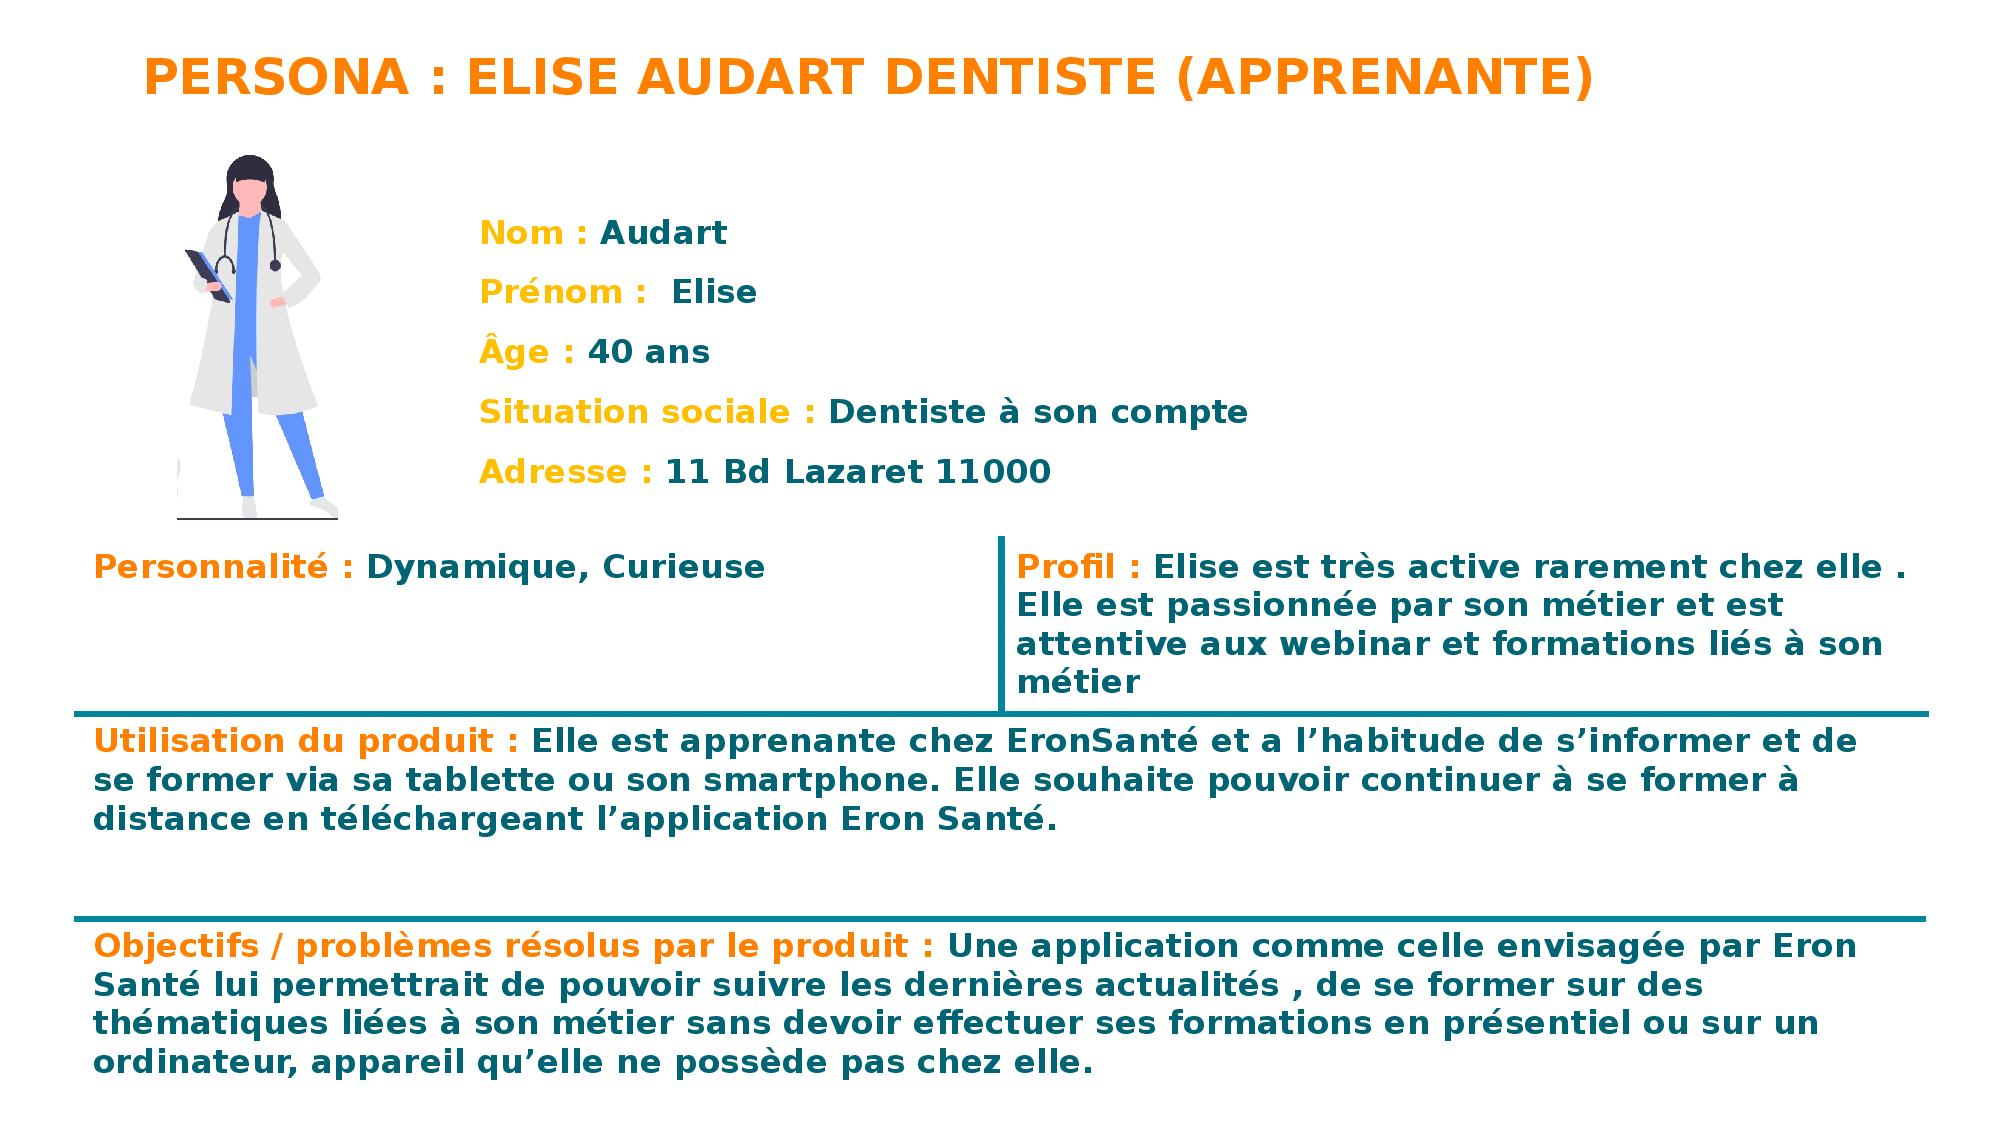
\includegraphics{../../Persona/Persona_Elise_Audart_Dentiste_Apprenante_Eron.jpg}

Fig.1 - Persona learner

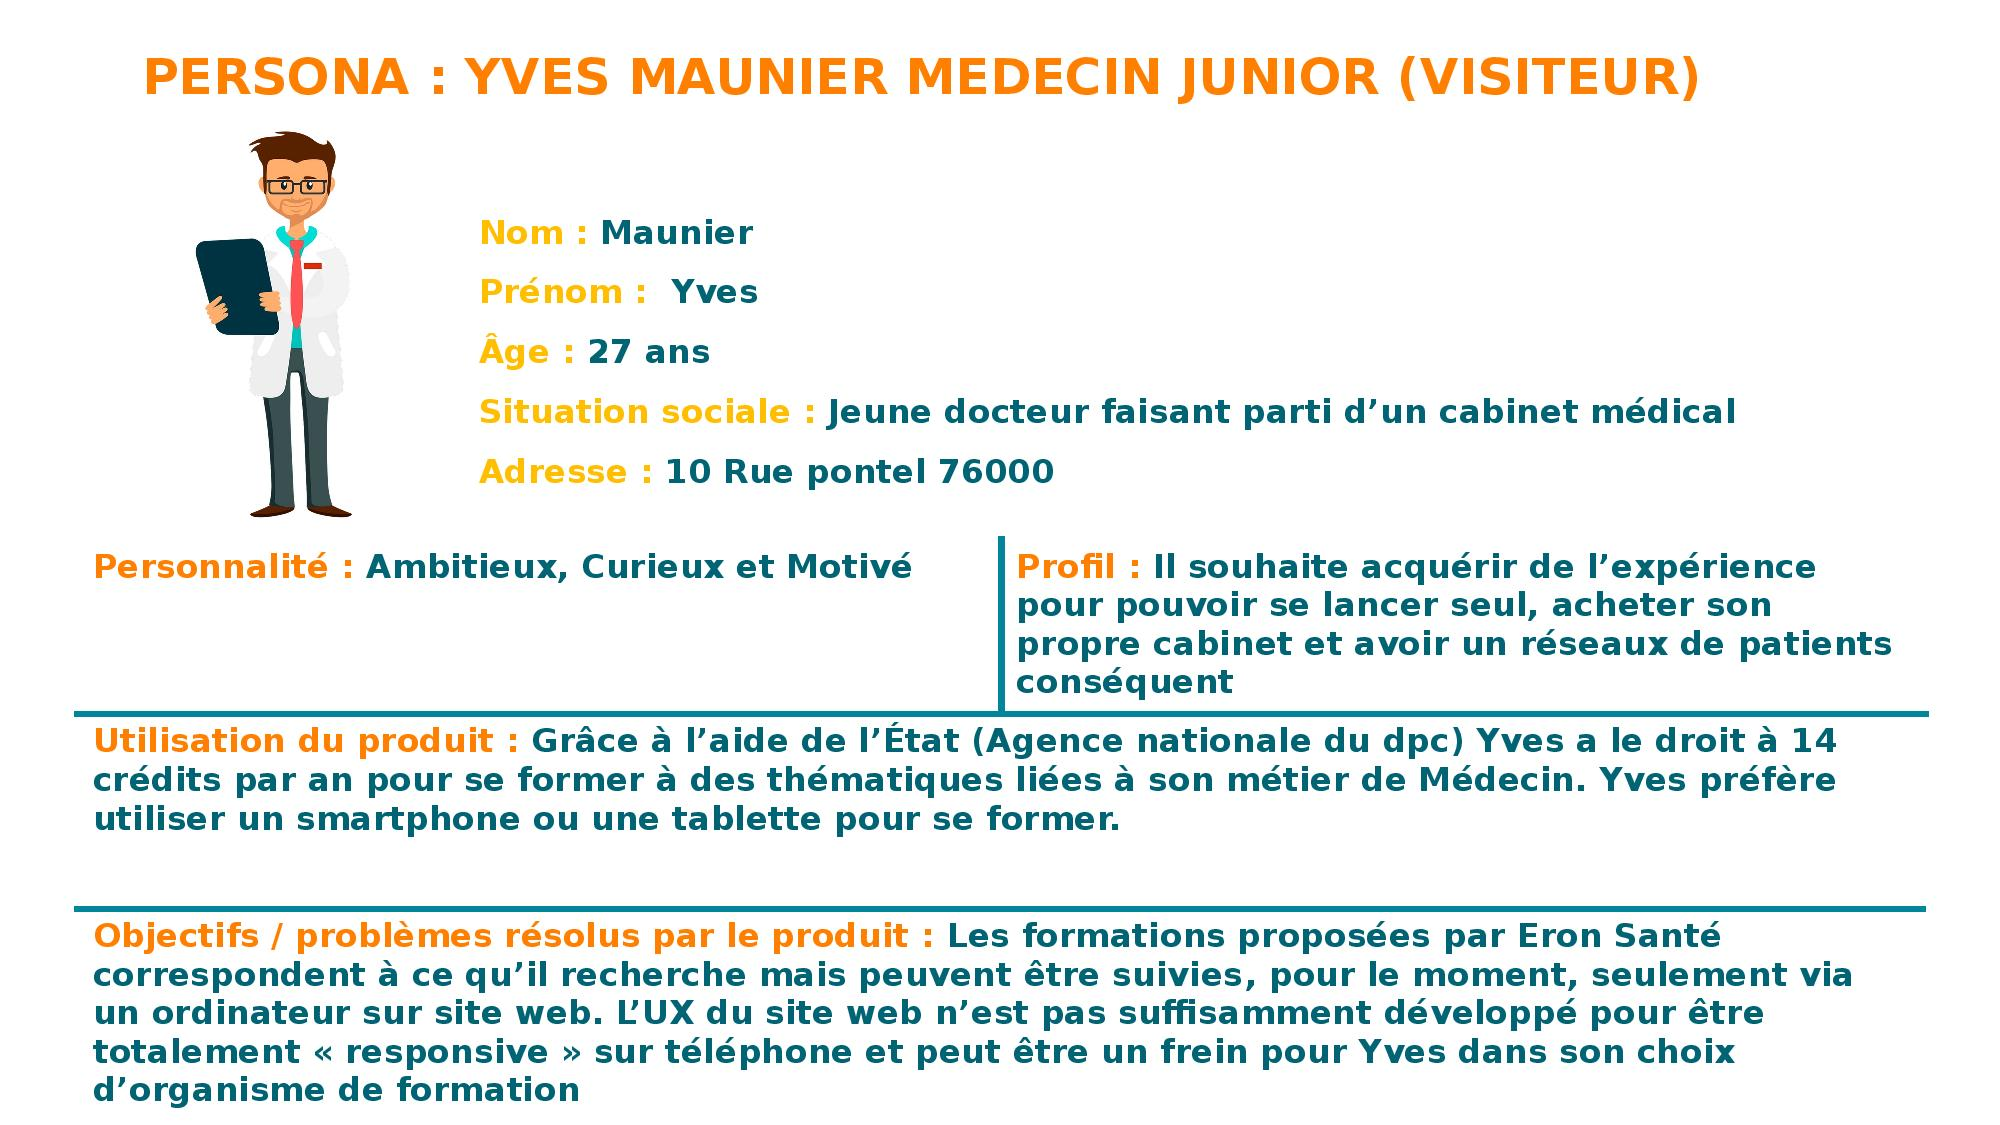
\includegraphics{../../Persona/Persona_Yves_Maunier_Medecin_Junior.jpg}

Fig.2 - Persona visitor

\hypertarget{to-discuss-and-to-validate}{%
\section{To discuss and to validate}\label{to-discuss-and-to-validate}}

\begin{longtable}[]{@{}
  >{\raggedright\arraybackslash}p{(\columnwidth - 14\tabcolsep) * \real{0.26}}
  >{\raggedright\arraybackslash}p{(\columnwidth - 14\tabcolsep) * \real{0.08}}
  >{\raggedright\arraybackslash}p{(\columnwidth - 14\tabcolsep) * \real{0.09}}
  >{\raggedright\arraybackslash}p{(\columnwidth - 14\tabcolsep) * \real{0.26}}
  >{\raggedright\arraybackslash}p{(\columnwidth - 14\tabcolsep) * \real{0.07}}
  >{\raggedright\arraybackslash}p{(\columnwidth - 14\tabcolsep) * \real{0.05}}
  >{\raggedright\arraybackslash}p{(\columnwidth - 14\tabcolsep) * \real{0.10}}
  >{\raggedright\arraybackslash}p{(\columnwidth - 14\tabcolsep) * \real{0.09}}@{}}
\toprule
Questions / Matter of discussion & Context of discussion & Category of
discussion & Author's question and role & Comments / Answer & State
(?,x,v) & Author's reviewer & Meeting's date to validate \\
\midrule
\endhead
Does the learner will get directly the training activated after the
payment ? & Wireframe's feedback & Screen/ UX / Wireframe &
Tiffany.j@eronservice / Backoffice & & ? & & \\
Another tab for shop to let the learner by training & Wireframe's
feedback & Screen/ UX / Wireframe & Tiffany.j@eronservice.fr /
Backofficedamien.v@eronservice.fr / Direction & yes & v & Damien Vert
and Andria Capai & 04/06/2021 \\
How precisely the learner could choose to be notified for deadline
training ? & Wireframe's feedback & Features / UX / Wireframe &
Tiffany.j@eronservice / Backoffice & & ? & & \\
\bottomrule
\end{longtable}

\hypertarget{external-ressources}{%
\section{External ressources}\label{external-ressources}}

\end{document}
